Hare and Hounds is a simple game with two players who alternate turns. One
player plays as the hare while the other plays as three hounds. The goal of the
hare is to escape the hounds while the goal of the hounds is to capture the
hare, this happens when the hare can not move on its turn. The board the game
is played on is shown in \autoref{fig:board}. The hounds player is only allowed
to move to adjacent squares that are to the right, either horizontally or
diagonally, they are also allowed to move vertically. Only one hound is allowed
to be moved in a turn. The hare can move in any direction to an adjacent
square. Only one piece is allowed to occupy a square at any time. The hare is
considered as escaped when it is to the left of the hounds. While this game
seems to be very simple it actually has quite deep strategy.

The game is also known as The Soldier's game, Game of Dwarfs, French Military
Game or any other regional equivalent. Not all of these variants use the same
shaped board but we'll focus on the board configuration shown in
\autoref{fig:board}. Other variations include longer or circular boards.

% Need to add more here

In this paper we will describe a method of learning to play the game of Hare
and Hounds using reinforcement learning. The methodology is explained in
\autoref{sec:method}, we discuss the results of training in
\autoref{sec:results} while final remarks are made in \autoref{sec:discussion}.

\begin{figure}[h]
	\centering
	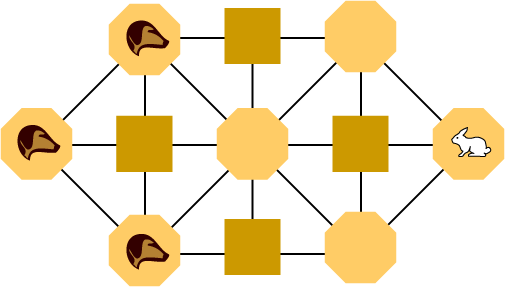
\includegraphics[width=.75\textwidth]{Hare_and_Hounds_board}
	\caption{The game board that Hare and Hounds is played on. The hare player
		starts on the right while the hounds player starts on the left.}
	\label{fig:board}
\end{figure}